\documentclass[a4paper,12pt]{article}
\usepackage[english]{babel}
\usepackage[utf8]{inputenc}

\usepackage[top=2.5cm, bottom=2.5cm, left=2cm, right=2cm]{geometry}

\usepackage{datetime}
\newdateformat{monthyeardate}{%
  \monthname[\THEMONTH], \THEYEAR}

% Math packages
\usepackage{mathtools}
\usepackage{amsmath}
\usepackage{amsfonts}
\usepackage{amssymb}

\usepackage{enumitem}
\usepackage{algorithm}
\usepackage{algpseudocode}

\usepackage{listings}

\usepackage{makecell}

\usepackage[hidelinks]{hyperref}

\title{Mobile and Social Sensing Systems}
\author{Francesco Barbarulo, Giovan Battista Rolandi}
\date{\monthyeardate\today}

\begin{document}
\pagenumbering{roman}

\maketitle
\abstract{The aim of these notes is to give some pills of every argument for the oral test. We have assumed that the reader has attended the lessons because these notes, by themselves, are not sufficient to have a global and profound knowledge.

We wish you good luck!}

\tableofcontents

\newpage

\pagenumbering{arabic}

\section{Introduction}
\subsection{Mobility}
\begin{itemize}
    \item \textbf{Physical}: hardware actually changes its physical position;
    \item \textbf{Logical}: applications and data may need to be moved for design reasons.
\end{itemize}

Mobile computing relys on the ability to use devices \textit{non-physically connected} and \textit{context-aware}. And these devices must keep computinal and communicaiton capabilities paying attention to energy comsumption because of their battery-powered nature.

\section{Localization systems}
Localization systems consist of two main blocks:
\begin{enumerate}[label=\roman*.]
	\item Set of deployed nodes with different \textit{states}:
		\begin{itemize}
		 	\item \textbf{beacon} (\textit{landmarks} or \textit{anchors}): already know their locations through a manual configuration or through GPS reading;
		  	\item \textbf{unknown} (\textit{targets}): do not have any information about their geographic locations;
		  	\item \textbf{settled}: targets nodes that has determined or estimated their locations.
		\end{itemize}
	\item Localization algorithm:
		\begin{itemize}
			\item GPS not longer used in CPS for cost and energy constraints;
			\item \textbf{GPS-free} techniques exploit the sensing and the wireless communication capabilities of CPS components.
		\end{itemize}
\end{enumerate}

\subsection{Topology}
The topology of a localization algorithm refers to \textit{where} and \textit{how} the location of a given node is calculated:

\begin{itemize}
	\item \textbf{Centralized localizaiton}: a central device estimates the location of unknown nodes based on the signal measurements forwarded by anchors;
	\item \textbf{Localized localization}: each object estimates its location using the collected signal measurements and location information of the anchor nodes in its neighbourhood.
\end{itemize}

We can distinguish four different system topologies for localization systems, as shown in Figure~\ref{fig:topology}.
\begin{figure}[H]
	\centering
  	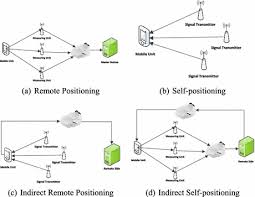
\includegraphics[width=0.4\textwidth]{img/topology}
  	\caption{\label{fig:topology}Taxonomy of localization systems topology}
\end{figure}

\subsection{Coordinate System}
\begin{itemize}
  \item \textbf{Physical}: locations are represented as a point in a 2D/3D coordinate system;
  \item \textbf{Symbolic}: locations are expressed as logical positions’ information;
  \item \textbf{Absolute}: locations are expressed as unique coordinate values making reference to \textit{anchor} nodes that know their positions;
  \item \textbf{Relative}: locations are determined relatively to other nodes with no reference to absolute anchors.
\end{itemize}

\subsection{Communication paradigm}
\begin{itemize}
  \item \textbf{Non-cooperative}: the communication is restricted between unknown nodes and anchors (\textit{high density} of anchors or \textit{long-range anchor transmissions} are needed);
  \item \textbf{Cooperative}: allows communication between unknown nodes (more \textit{processing} is required);
  \item \textbf{Opportunistic}: exploits interactions between nodes that occasionally pass each other in their proximity (efficient \textit{node discovery} and \textit{data exchange}).
\end{itemize}

\subsection{Performance metrics}
\begin{itemize}
  \item \textbf{Accuracy}: mean (Euclidean) distance error between the estimated location and the true location;
  \item \textbf{Precision}: variation over many algorithm trials, CDF of distance error;
  \item \textbf{Complexity}: hardware and/or software;
  \item \textbf{Robustness}: behavior under unwanted conditions;
  \item \textbf{Scalability}: geographical and density;
  \item \textbf{Cost}
\end{itemize}



\end{document}